\section{Motion Generation Experiments}
\label{sec:vimo_exps}

\paragraph{Implementation details.}
Training used the ADAN optimizer with an initial learning rate of $1 \times 10^{-4}$. Sequences were resampled from 60 FPS to 30 FPS, yielding $S=150$ frames per five-second clip. Diffusion timesteps used $T=1000$, with DDIM acceleration during sampling. SMPL axis-angle parameters were converted to 6D rotations using orthogonalization~\cite{6drot2020}. Foot-contact labels were derived from near-zero vertical foot and toe velocities. Training followed the AIST++ protocol~\cite{aist2021}: break and middle hip-hop genres were held out for testing, while the remaining genres were used for training. Multi-view 2D keypoints served as conditioning input, and batch size was fixed at 32. The objective of these experiments was not only to train the generator in isolation, but also to verify that its outputs can be converted into reference motions suitable for physically simulated control.

\begin{figure}[htbp]
    \centering
    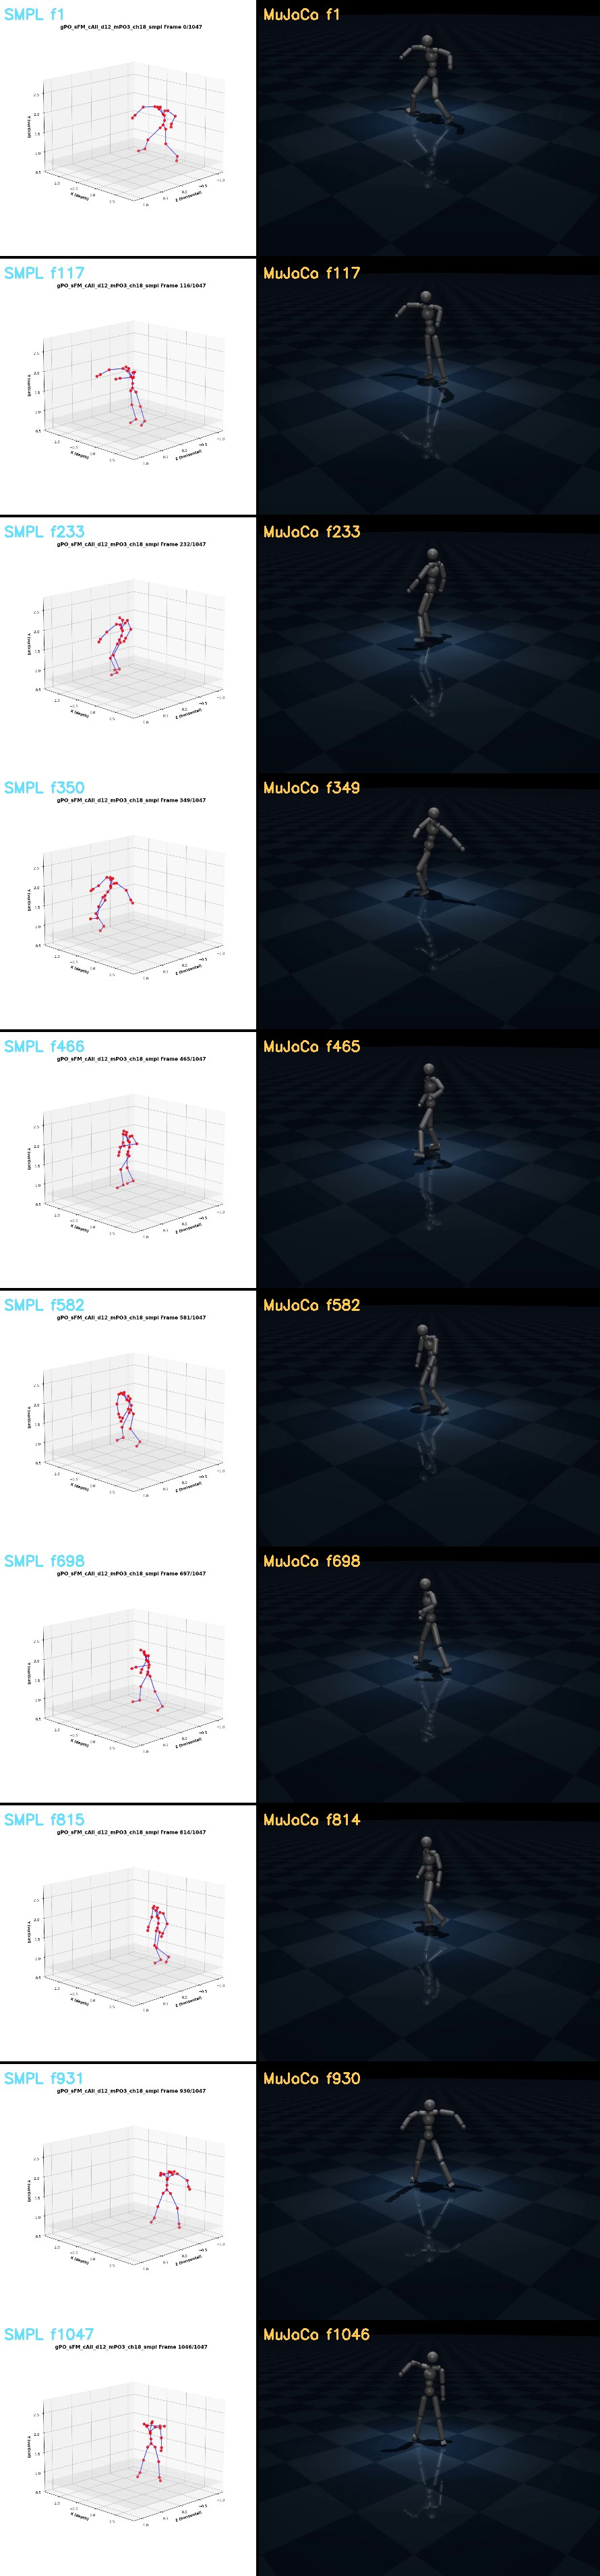
\includegraphics[height=.95\textheight, keepaspectratio]{Pictures/sample_conversion.jpg}
    \caption{SMPL Humanoid (34-joints) to Deepmimic Humanoid (28-joints) Retargeted Sample}
    \label{fig:smpl_exp}
\end{figure}

\paragraph{Training stability and lambda scheduling.}
Early epochs set $\lambda_{\text{joints}}=0.01$, $\lambda_{\text{vel}}=1.0$, $\lambda_{\text{foot}}=0.1$. The velocity loss dominated, causing collapse to static poses where $\mathbf{R}_{t+1} \approx \mathbf{R}_t$. Direct matrix subtraction $\mathbf{R}_{t+1} - \mathbf{R}_t$ is not physically meaningful on $SO(3)$ and produced large gradients that overwhelmed the diffusion objective. The model learned that predicting no motion minimized loss.

To counteract collapse, lambda scheduling evolved: $\lambda_{\text{joints}}$ increased to $0.1$ by epoch 25, $\lambda_{\text{vel}}$ reduced to $0.01$ by epoch 40, and $\lambda_{\text{foot}}$ rose to $0.5$. Crucially, setting any auxiliary loss to zero caused immediate mean-pose collapse; all three losses required non-zero weights from initialization. The final stable configuration used $\lambda_{\text{joints}}=0.1$, $\lambda_{\text{vel}}=0.02$, $\lambda_{\text{foot}}=0.05$.

\paragraph{SNR weighting strategies.}
Standard diffusion training with constant weighting $w_t=1$ yielded poor sample efficiency because most late timesteps contributed negligible gradient after the SNR cliff. Experiments evaluated four strategies:
\begin{itemize}
    \item \textbf{Min-cap}: $w_t = \min(\text{SNR}_t, \gamma)$ with $\gamma=1$ created a steep cliff; 70\% of steps carried near-zero weight.
    \item \textbf{Decay min-cap}: Linear or sqrt decay schedules smoothed early steps but left the cliff intact.
    \item \textbf{Averaging}: $w_t = \frac{1}{2}[\min(\text{SNR}_t, 1) + \sqrt{1-t/T}]$ filled the dead zone, achieving ~50\% sample efficiency. This variant prevented collapse and maximized data utilization.
    \item \textbf{Normalization}: Per-batch normalization of $w_t$ stabilized training but slowed convergence when combined with high caps ($\gamma=2$).
\end{itemize}
The most stable setting used square-root decay averaging with $\gamma=1$ and no per-batch normalization, providing the best trade-off between gradient coverage and convergence speed~\cite{minsnr2024}.

\begin{figure}[htbp]
\centering
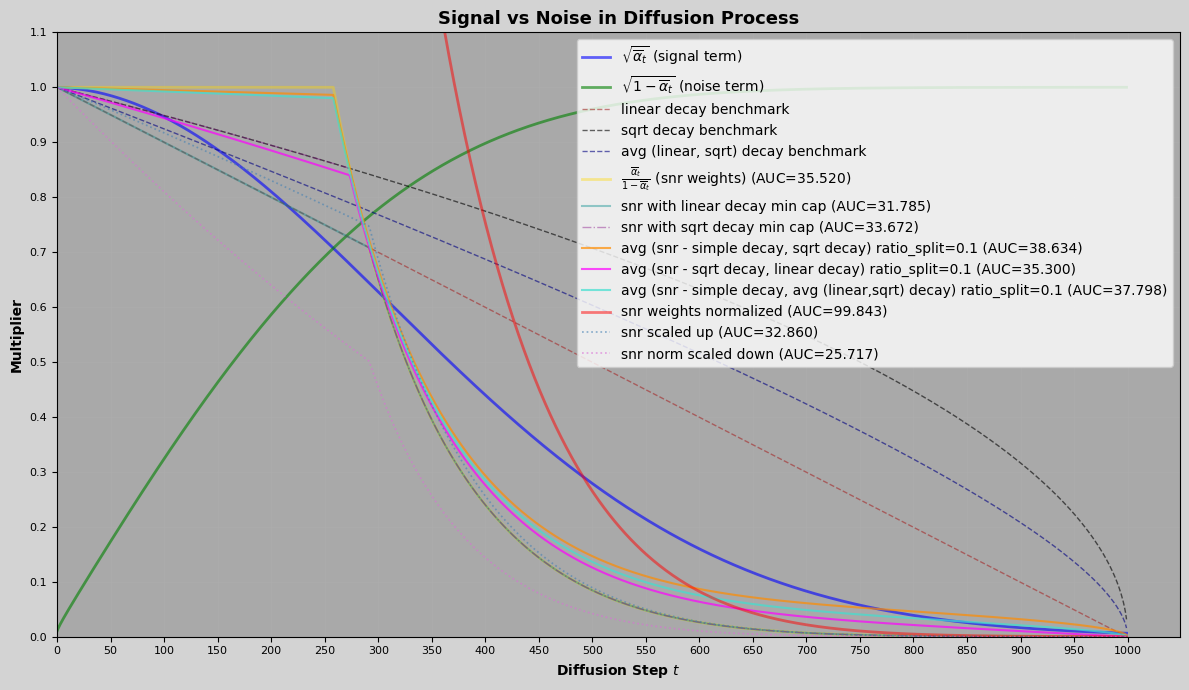
\includegraphics[width=\textwidth]{Pictures/snr.png}
\caption{Ablation of SNR weighting strategies for a $T=1000$ linear diffusion process ($\beta \in [1e-4, 0.02]$). Plotted are the signal term $\sqrt{\bar{\alpha}_t}$ and noise term $\sqrt{1-\bar{\alpha}_t}$, benchmark decay curves (linear, square root, and their average), and proposed SNR variants: simple ratio $\frac{\bar{\alpha}_t}{1-\bar{\alpha}_t}$, min-capped decays, ratio-split=0.1 blends, normalized, and scaled weights. Area-under-curve (AUC) percentages (cap=1.0) quantify integrated weight magnitude. Normalized SNR achieves the highest AUC (99.843\%), while simple SNR decays precipitously.}
\label{fig:snr}
\end{figure}

\paragraph{Temporal modeling with PTSS.}
Vectorized timesteps enable frame-wise noise schedules but risk combinatorial explosion. Probabilistic Timestep Sampling Strategy (PTSS) controls complexity. Experiments varied $p$, the probability of independent per-frame sampling:
\begin{itemize}
    \item $p=0.2$ to $0.5$ over epochs 1–50 showed steady loss decrease and growing prediction variance.
    \item $p>0.6$ introduced excessive variance, triggering SMPL forward kinematics violations in root position scale.
    \item Returning to $p=0.2$ after epoch 60 with learning rate increased to $2.5 \times 10^{-4}$ stabilized training.
\end{itemize}
PTSS improved temporal flexibility but required careful scheduling. In practice, low initial values of $p$ were essential for stability, while larger values were useful only after the model had already learned coarse motion structure~\cite{ptss2024}.

\paragraph{Model architecture ablations.}
Two FiLM implementations were compared. Version~1 shared a single linear layer across all modulation points within a denoiser block. Version~2 used three separate linear layers for self-attention, cross-attention, and MLP outputs. Both applied identical parameters across frames.
\begin{itemize}
    \item Small models ($d=128$, $n_{\text{heads}}=4$) showed no performance gap.
    \item Large models ($d=256$, $n_{\text{heads}}=8$) revealed Version~2 converged marginally slower due to increased parameters.
    \item Version~1 was selected for production runs as parameter reduction mitigated overfitting on the 26k-sample dataset.
    \item The difference was negligible; architectural novelty lies in conditioning strategy, not FiLM multiplicity.
\end{itemize}

\paragraph{Convergence monitoring and deployment use.}
Tracking loss component magnitudes guided training:
\begin{itemize}
    \item $\mathcal{L}_{\text{joints}}$ target: 0.01–0.02. Below 0.01 indicated overfitting; above 0.03 required higher $\lambda_{\text{joints}}$.
    \item $\mathcal{L}_{\text{vel}}$ target: 0.05–0.10. Below 0.01 signaled static predictions; above 0.15 produced erratic motion.
    \item $\mathcal{L}_{\text{foot}}$ target: $10^{-4}$–$10^{-3}$. Above 0.01 revealed excessive foot sliding; below $10^{-4}$ over-constrained naturalness.
\end{itemize}
Prediction standard deviation steadily increased from near-zero to stable values around 0.1--0.2, confirming the emergence of dynamic motion. Beyond quantitative convergence, the important pipeline-level outcome was successful retargeting of generated clips into simulation-ready references. This was verified on multiple converted motion families, including checkpoints corresponding to `gBR`, `gHO`, `gJS`, `gLH`, `gLO`, `gMH`, and `gPO`, which were used as motion inputs for downstream control experiments.

\section{ViMo-Flow: Qualitative Results}
\label{sec:vimo_results}

Two transformer-diffusion configurations are evaluated: small model (\(d_{\text{model}} = 128\), \(n_{\text{heads}} = 4\)) and big model (\(d_{\text{model}} = 256\), \(n_{\text{heads}} = 8\)). Each run shows ground-truth reference frames, deterministic denoising predictions \(\hat{\mathbf{x}}_0\) at selected timesteps, and stochastic generation samples.

\paragraph{\textbf{Small model v1, no PTSS (ViMo baseline), 50 epochs}}

\begin{figure}[H]
    \centering
    
\includegraphics[width=\textwidth]{outputs/d128_h4/run_v1_warm50/ground_truth_frames.png}
    \caption{Ground-truth motion sequence (small model v1, no PTSS).}
    \label{fig:run_v1_warm50_ground_truth_frames}
\end{figure}

\begin{figure}[H]
    \centering
    
\includegraphics[width=\textwidth]{outputs/d128_h4/run_v1_warm50/predicted_estimate_frames.png}
    \caption{Deterministic predictions \(\hat{\mathbf{x}}_0\) at timesteps
    \(t \in \{100, 200, 300, 400, 500\}\) (small model v1, no PTSS).}
    \label{fig:run_v1_warm50_predicted_estimates}
\end{figure}

\begin{figure}[H]
    \centering
\includegraphics[width=\textwidth]{outputs/d128_h4/run_v1_warm50/stochastic_generation_frames.png}
    \caption{Stochastic samples at timesteps
    \(t \in \{100, 200, 300, 400, 500\}\) (small model v1, no PTSS).}
    \label{fig:run_v1_warm50_stochastic_generations}
\end{figure}

%%%%%%%%%%%%%%%%%%%%%%%%%%%%%%%%%%%%%%%%%%%%%%%%%%%%%%%%%%%%%%%%%%%%%

\paragraph{\textbf{Small model v1 with PTSS, 65 epochs}}

\begin{figure}[H]
    \centering
    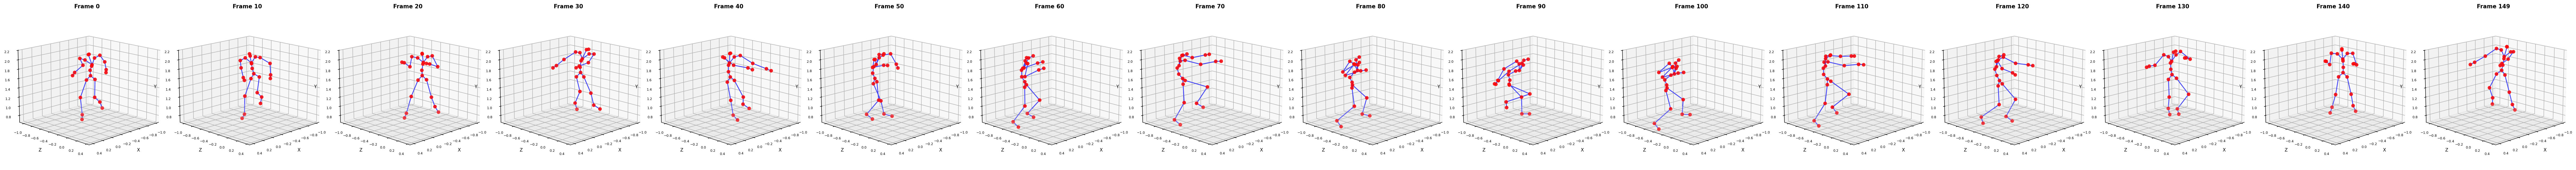
\includegraphics[width=\textwidth]{outputs/d128_h4/run_v1(sq)_ptss/ground_truth_frames.png}
    \caption{Ground-truth motion sequence (small model v1, PTSS).}
    \label{fig:run_v1sq_PTSS_ground_truth_frames}
\end{figure}

\begin{figure}[H]
    \centering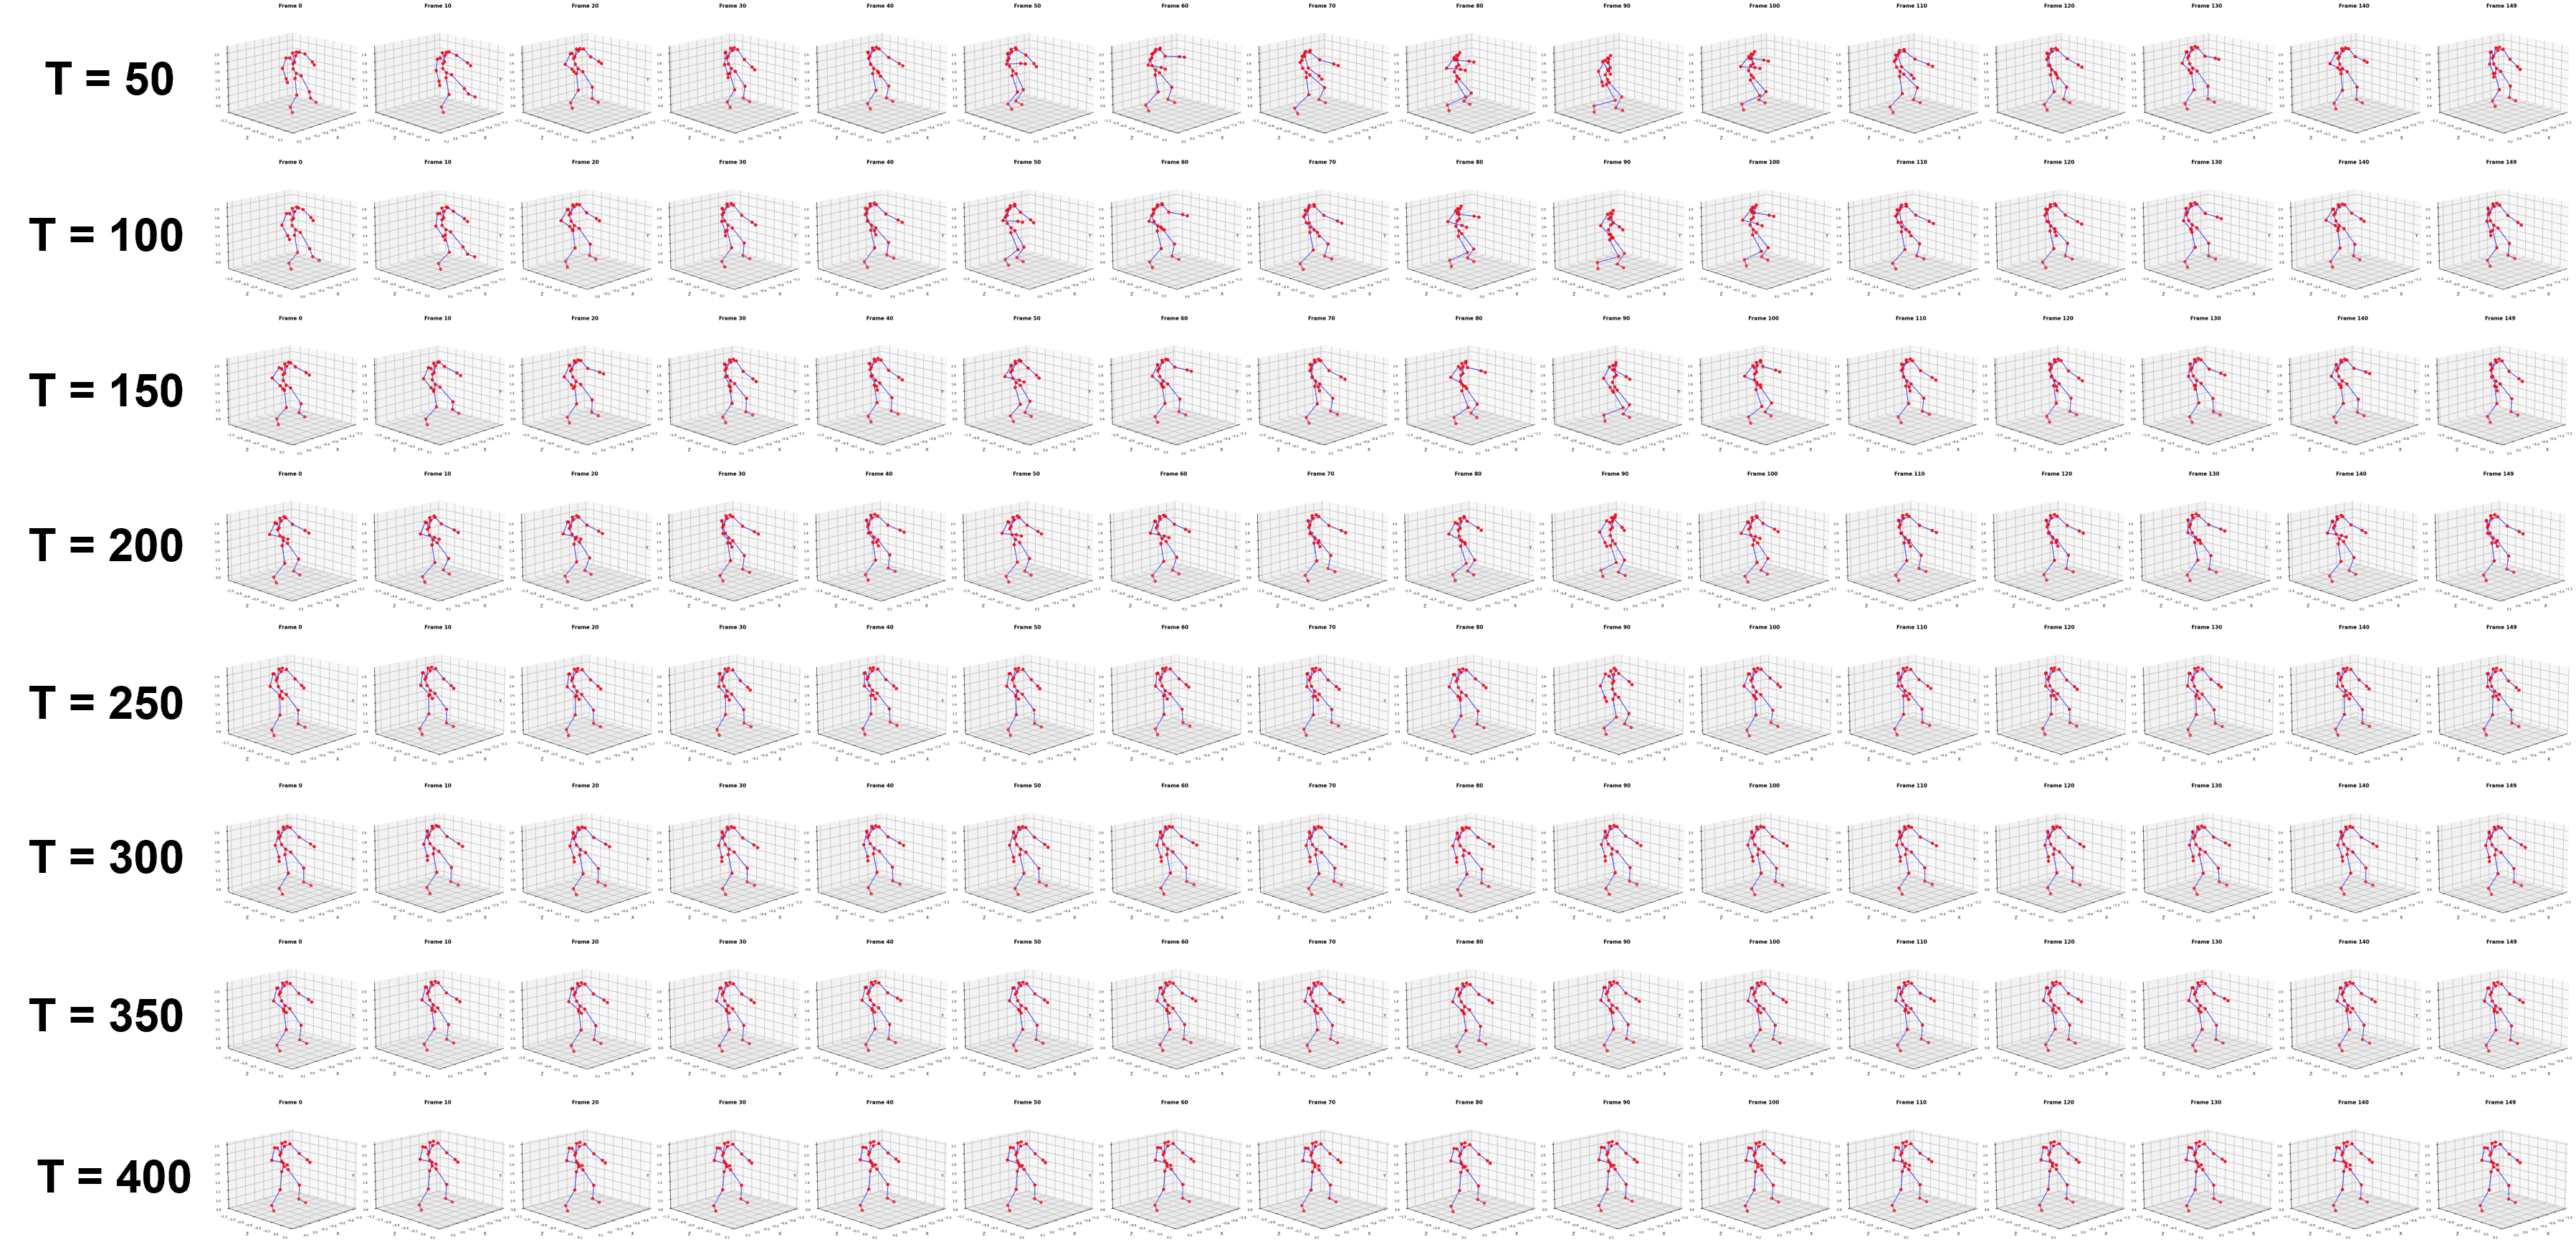
\includegraphics[width=\textwidth]{outputs/d128_h4/run_v1(sq)_ptss/predicted_estimate_frames.png}
    \caption{Deterministic predictions \(\hat{\mathbf{x}}_0\) at
    \(t \in \{50, 100, 150, 200, 250, 300, 350, 400\}\) (small model v1, PTSS).}
    \label{fig:run_v1sq_PTSS_predicted_estimates}
\end{figure}

\begin{figure}[H]
    \centering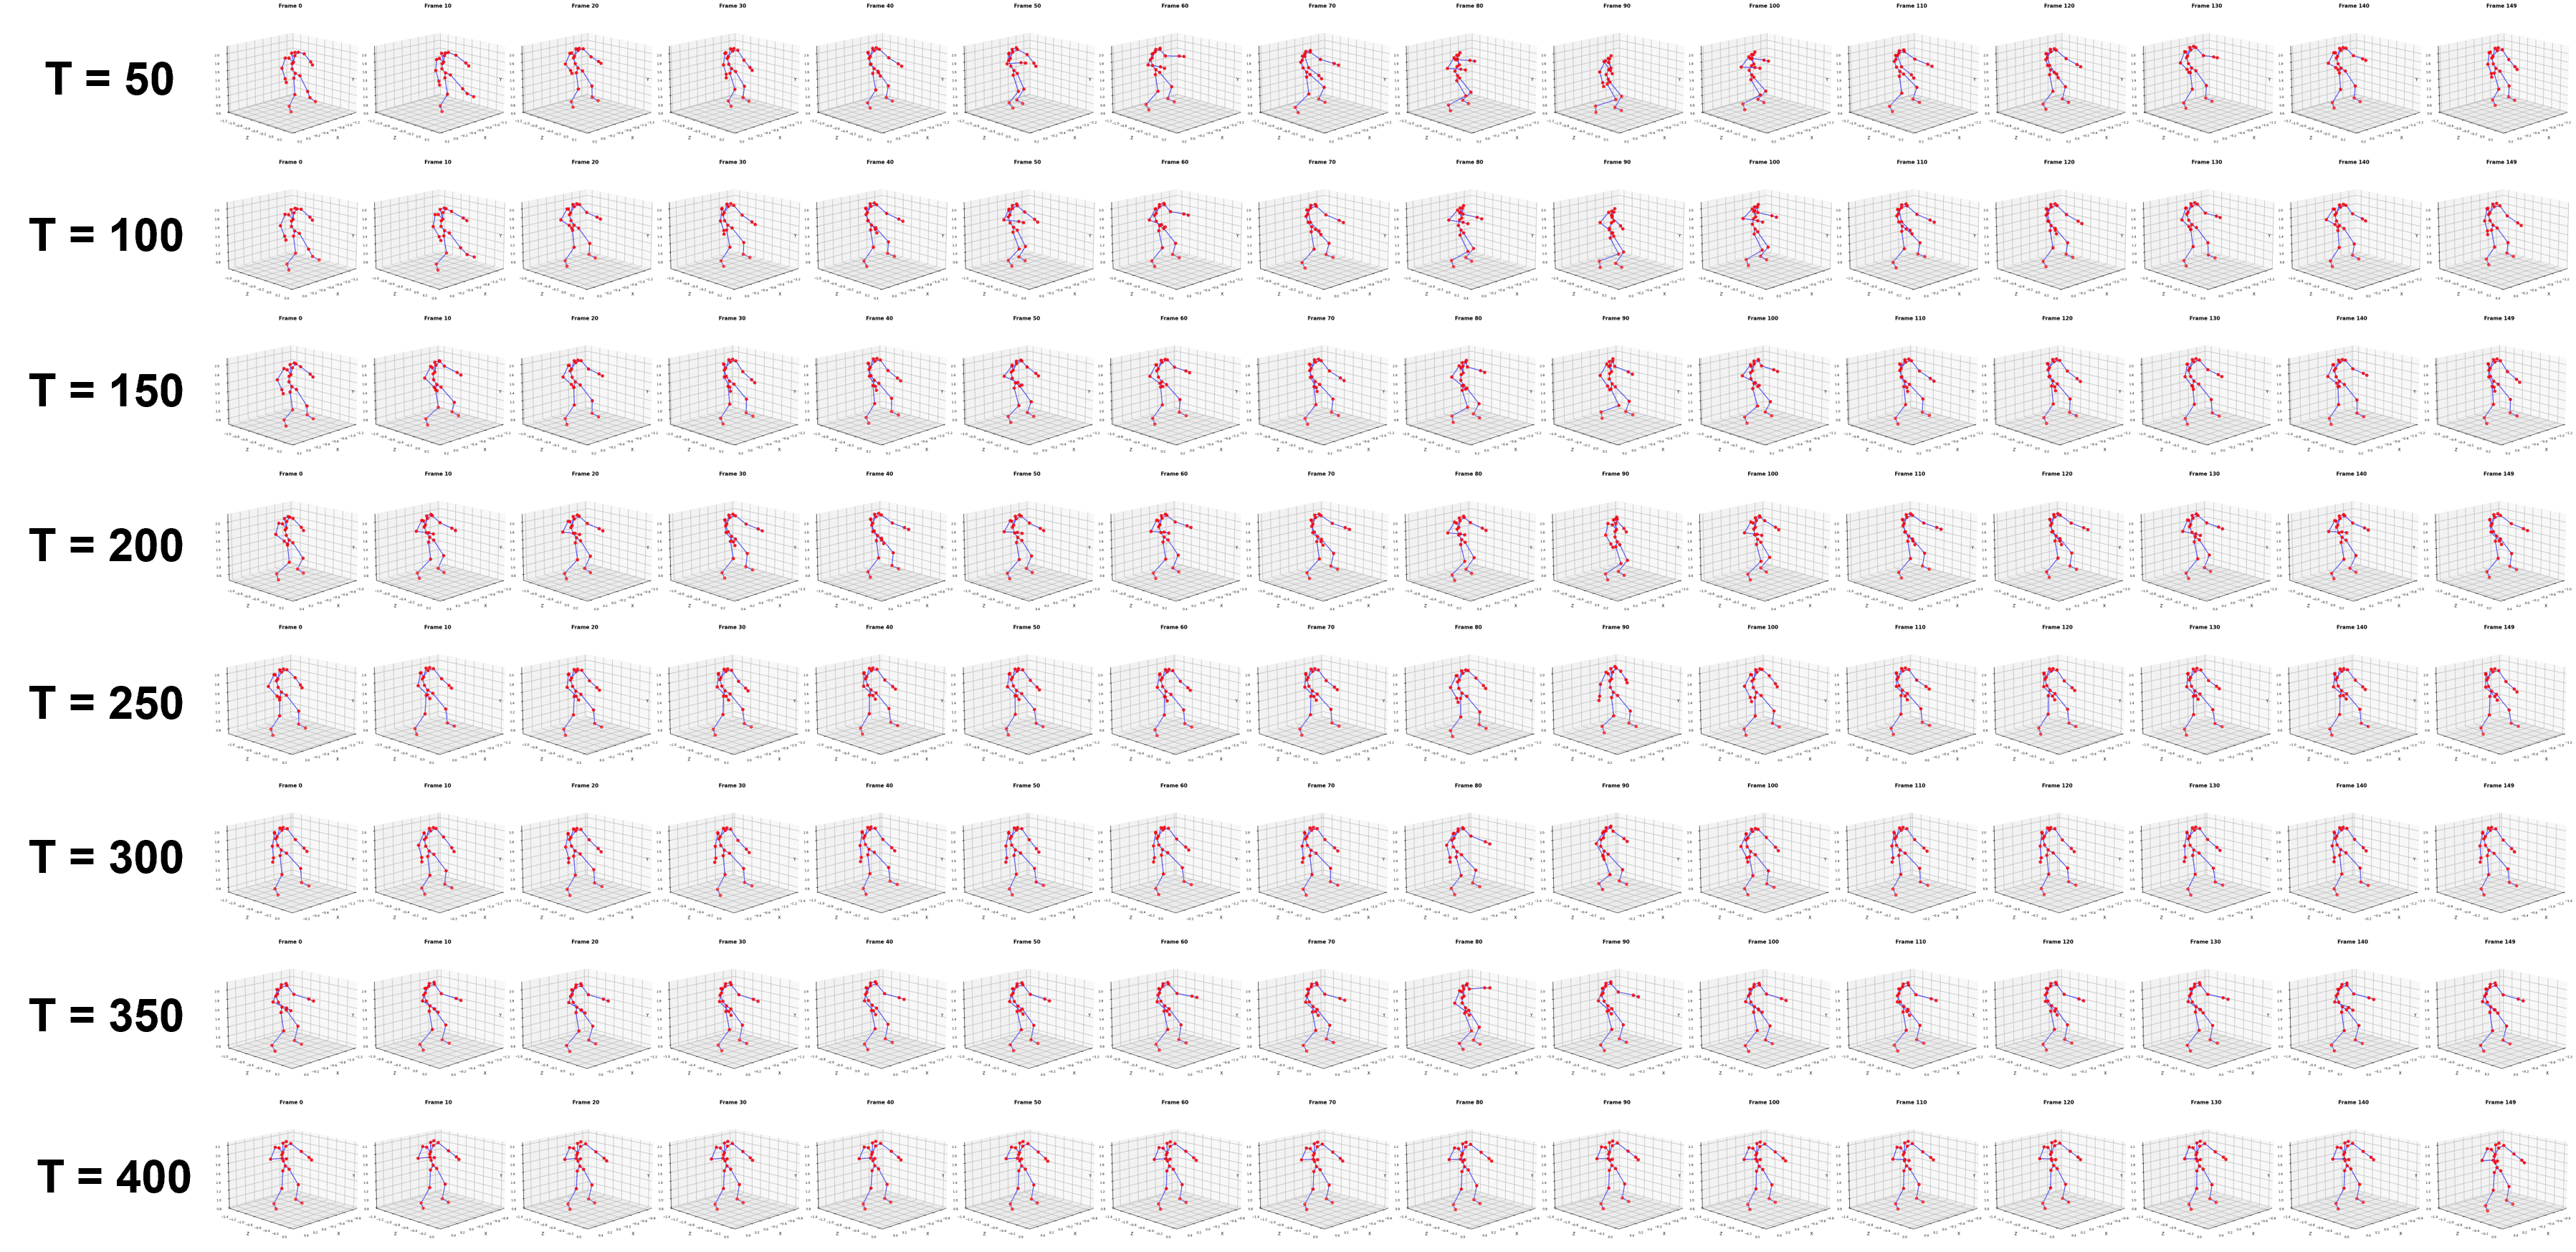
\includegraphics[width=\textwidth]{outputs/d128_h4/run_v1(sq)_ptss/stochastic_generation_frames.png}
    \caption{Stochastic samples at
    \(t \in \{50, 100, 150, 200, 250, 300, 350, 400\}\) (small model v1, PTSS).}
    \label{fig:run_v1sq_PTSS_stochastic_generations}
\end{figure}

%%%%%%%%%%%%%%%%%%%%%%%%%%%%%%%%%%%%%%%%%%%%%%%%%%%%%%%%%%%%%%%%%%%%%

\paragraph{\textbf{Small model v2 with PTSS, 65 epochs}}

\begin{figure}[H]
    \centering
\includegraphics[width=\textwidth]{outputs/d128_h4/run_v2(sq)_ptss/ground_truth_frames.png}
    \caption{Ground-truth motion sequence (small model v2, PTSS).}
    \label{fig:run_v2sq_PTSS_ground_truth_frames}
\end{figure}

\begin{figure}[H]
    \centering
\includegraphics[width=\textwidth]{outputs/d128_h4/run_v2(sq)_ptss/predicted_estimate_frames.png}
    \caption{Deterministic predictions \(\hat{\mathbf{x}}_0\) at
    \(t \in \{50, 100, 150, 200, 250\}\) (small model v2, PTSS).}
    \label{fig:run_v2sq_PTSS_predicted_estimates}
\end{figure}

\begin{figure}[H]
    \centering
\includegraphics[width=\textwidth]{outputs/d128_h4/run_v2(sq)_ptss/stochastic_generation_frames.png}
    \caption{Stochastic samples at
    \(t \in \{50, 100, 150, 200, 250\}\) (small model v2, PTSS).}
    \label{fig:run_v2sq_PTSS_stochastic_generations}
\end{figure}

%%%%%%%%%%%%%%%%%%%%%%%%%%%%%%%%%%%%%%%%%%%%%%%%%%%%%%%%%%%%%%%%%%%%%

\paragraph{\textbf{Big model v1 with PTSS, 100 epochs}}

\begin{figure}[H]
    \centering
    
\includegraphics[width=\textwidth]{outputs/d256_h8/run_v1(sq) PTSS/ex1/ground_truth_frames.png}
    \caption{Example 1: ground-truth motion sequence (big model v1, PTSS).}
    \label{fig:d256_h8_ex1_ground_truth_frames}
\end{figure}

\begin{figure}[H]
    \centering
    
\includegraphics[width=\textwidth]{outputs/d256_h8/run_v1(sq) PTSS/ex1/predicted_estimate_frames.png}
    \caption{Example 1: deterministic predictions \(\hat{\mathbf{x}}_0\) at
    \(t \in \{50, 100, 150, 200, 250, 300, 350, 400, 450\}\) (big model v1, PTSS).}
    \label{fig:d256_h8_ex1_predicted_estimates}
\end{figure}

\begin{figure}[H]
    \centering
    
\includegraphics[width=\textwidth]{outputs/d256_h8/run_v1(sq) PTSS/ex1/stochastic_generation_frames.png}
    \caption{Example 1: stochastic samples at
    \(t \in \{50, 100, 150, 200, 250, 300, 350, 400, 450\}\) (big model v1, PTSS).}
    \label{fig:d256_h8_ex1_stochastic_generations}
\end{figure}

\begin{figure}[H]
    \centering
    
\includegraphics[width=\textwidth]{outputs/d256_h8/run_v1(sq) PTSS/ex2/ground_truth_frames.png}
    \caption{Example 2: ground-truth motion sequence (big model v1, PTSS).}
    \label{fig:d256_h8_ex2_ground_truth_frames}
\end{figure}

\begin{figure}[H]
    \centering
    
\includegraphics[width=\textwidth]{outputs/d256_h8/run_v1(sq) PTSS/ex2/predicted_estimate_frames.png}
    \caption{Example 2: deterministic predictions \(\hat{\mathbf{x}}_0\) at
    \(t \in \{50, 100, 150, 200, 250, 300, 350\}\) (big model v1, PTSS).}
    \label{fig:d256_h8_ex2_predicted_estimates}
\end{figure}

\begin{figure}[H]
    \centering
    
\includegraphics[width=\textwidth]{outputs/d256_h8/run_v1(sq) PTSS/ex2/stochastic_generation_frames.png}
    \caption{Example 2: stochastic samples at
    \(t \in \{50, 100, 150, 200, 250, 300, 350\}\) (big model v1, PTSS).}
    \label{fig:d256_h8_ex2_stochastic_generations}
\end{figure}


